\subsection{Timeline}

\begin{frame}{}
\vspace{-3.47em}
\begin{figure}[!htb]
    \begin{tikzpicture}[scale=0.8]
        \draw[->, line width=1pt] (-1.5, 6.0)
        -- ++(1.5, 0.0) node[above] {2019.04}
        -- ++(1.5, 0.0) node[above] {2019.08}
        -- ++(1.5, 0.0) node[above] {2019.12}
        -- ++(1.5, 0.0) node[above] {2020.04}
        -- ++(1.5, 0.0) node[above] {2020.08}
        -- ++(1.5, 0.0) node[above] {2020.12}
        -- ++(1.5, 0.0) node[above] {2021.04}
        -- ++(1.5, 0.0) node[above] {2021.08}
        -- ++(1.5, 0.0) node[above] {2021.12}
        -- ++(1.5, 0.0) node[above] {2022.04}
        -- ++(1.5, 0.0);
        \draw[fill=black] (0.0, 6.0) circle (2pt);
        \draw[fill=black] (1.5, 6.0) circle (2pt);
        \draw[fill=black] (3.0, 6.0) circle (2pt);
        \draw[fill=black] (4.5, 6.0) circle (2pt);
        \draw[fill=black] (6.0, 6.0) circle (2pt);
        \draw[fill=black] (7.5, 6.0) circle (2pt);
        \draw[fill=black] (9.0, 6.0) circle (2pt);
        \draw[fill=black] (10.5, 6.0) circle (2pt);
        \draw[fill=black] (12.0, 6.0) circle (2pt);
        \draw[fill=black] (13.5, 6.0) circle (2pt);
        \draw[line width=1pt] (0.75, 6.0) -- (0.75, 5.5);
        \draw[line width=1pt] (2.25, 6.0) -- (2.25, 4.5);
        \draw[line width=1pt] (3.75, 6.0) -- (3.75, 3.5);
        \draw[line width=1pt] (4.5, 6.0) -- (4.5, 7);
        \node[text width=\textwidth,anchor=north west,fill=white,opacity=.6,text opacity=1] at (-1.5, 5.5) {Towards large deformation: formulate a set of hyperelastic potentials with tension-compression asymmetry and qualitatively evaluate their performance in the context of dynamic fracture.};
        \node[text width=\textwidth,anchor=north west,fill=white,opacity=.6,text opacity=1] at (-1.5, 4.5) {Coupling with plasticity: formulate a thermodynamically consistent model for coupled elasticity, plasticity and fracture.};
        \node[text width=\textwidth,anchor=north west,fill=white,opacity=.6,text opacity=1] at (-1.5, 3.5) {Investigate the impact of several constitutive choices in the elastic-plastic-fracture coupled model.};
        \node[anchor=south] at (4.5, 7) {\textcolor{yellow}{\faStar} Prelim};
    \end{tikzpicture}
\end{figure}
\end{frame}

\begin{frame}{}
\vspace{-3em}
\begin{figure}[!htb]
    \begin{tikzpicture}[scale=0.8]
        \draw[->, line width=1pt] (-1.5, 6.0)
        -- ++(1.5, 0.0) node[above] {2019.04}
        -- ++(1.5, 0.0) node[above] {2019.08}
        -- ++(1.5, 0.0) node[above] {2019.12}
        -- ++(1.5, 0.0) node[above] {2020.04}
        -- ++(1.5, 0.0) node[above] {2020.08}
        -- ++(1.5, 0.0) node[above] {2020.12}
        -- ++(1.5, 0.0) node[above] {2021.04}
        -- ++(1.5, 0.0) node[above] {2021.08}
        -- ++(1.5, 0.0) node[above] {2021.12}
        -- ++(1.5, 0.0) node[above] {2022.04}
        -- ++(1.5, 0.0);
        \draw[fill=black] (0.0, 6.0) circle (2pt);
        \draw[fill=black] (1.5, 6.0) circle (2pt);
        \draw[fill=black] (3.0, 6.0) circle (2pt);
        \draw[fill=black] (4.5, 6.0) circle (2pt);
        \draw[fill=black] (6.0, 6.0) circle (2pt);
        \draw[fill=black] (7.5, 6.0) circle (2pt);
        \draw[fill=black] (9.0, 6.0) circle (2pt);
        \draw[fill=black] (10.5, 6.0) circle (2pt);
        \draw[fill=black] (12.0, 6.0) circle (2pt);
        \draw[fill=black] (13.5, 6.0) circle (2pt);
        \draw[line width=1pt] (4.5, 6.0) -- (4.5, 7);
        \draw[line width=1pt] (9.0, 6.0) -- (9.0, 7);
        \draw[line width=1pt] (13.5, 6.0) -- (13.5, 7);
        \draw[line width=1pt] (5.25, 6.0) -- (5.25, 5.5);
        \draw[line width=1pt] (6.75, 6.0) -- (6.75, 5.0);
        \draw[line width=1pt] (8.25, 6.0) -- (8.25, 4.0);
        \draw[line width=1pt] (9.75, 6.0) -- (9.75, 2.5);
        \draw[line width=1pt] (11.25, 6.0) -- (11.25, 1.0);
        \draw[line width=1pt] (12.75, 6.0) -- (12.75, 0.0);
        \node[anchor=south] at (4.5, 7) {\textcolor{yellow}{\faStar} Prelim};
        \node[anchor=south] at (9.0, 7) {\textcolor{blue}{\faStar} Midterm?};
        \node[anchor=south] at (13.5, 7) {\textcolor{red}{\faStar} Dissertation};
        \node[text width=\textwidth,anchor=north west,fill=white,opacity=.6,text opacity=1] at (-1.5, 5.5) {Formulate and implement the phase-field fracture model based on the fourth-order Cahn-Hilliard theory.};
        \node[text width=\textwidth,anchor=north west,fill=white,opacity=.6,text opacity=1] at (-1.5, 5.0) {Incorporate thermal effects, e.g. thermal expansion, thermal softening, heat transfer across weak discontinuities.};
        \node[text width=\textwidth,anchor=north west,fill=white,opacity=.6,text opacity=1] at (-1.5, 4.0) {Investigate the effect of model hyperparameters on macroscopic responses. Foreseeable parameters include regularization length(s), parameters in the plastic-hardening law, parameters in the cohesive traction-separation law, parameters in the thermal softening law, etc..};
        \node[text width=\textwidth,anchor=north west,fill=white,opacity=.6,text opacity=1] at (-1.5, 2.5) {Apply the model to simulate the Kalthoff-Winkler problem. Other problems, e.g. those from past Sandia fracture challenges, are also applicable where plasticity and thermal effects have proven to be critical in predicting the correct material response.};
        \node[text width=\textwidth,anchor=north west,fill=white,opacity=.6,text opacity=1] at (-1.5, 1.0) {Wrap-up. Review (or even reformulate if necessary) previous modeling choices given previously obtained results.};
        \node[text width=\textwidth,anchor=north west,fill=white,opacity=.6,text opacity=1] at (-1.5, 0.0) {Formulate the phase-field fracture problem without any arbitrary split in the elastic energy. Instead, explore other possibilities in enforcing the contact conditions between fracture surfaces.};
    \end{tikzpicture}
\end{figure}
\end{frame}
